\documentclass{article}
\usepackage{fullpage,graphicx,amsmath,setspace}
\begin{document}

\doublespace

  \begin{center}
  \begin{huge}
$\alpha$-emitting mineral inclusions in apatite, their effect
on (U-Th)/He ages, and how to reduce it\\
  \end{huge}
\vspace{0.2cm}
%\texttt{(revised version - Aug 8, 2006)}\\
%\vspace{0.2cm}
Pieter Vermeesch\footnote[1]{Institute of Isotope Geology and
Mineral Resources, ETH-Z\"{u}rich, Switzerland},
Diane Seward\footnote[2]{Geological Institute, ETH-Z\"{u}rich, Switzerland},
Christopher Latkoczy\footnote[3]{Laboratory of Inorganic Chemistry,
ETH-Z\"{u}rich, Switzerland}\\
Martin Wipf$^2$, Detlef G\"{u}nther$^3$ and Heinrich Baur$^1$
\vspace{0.2cm}
  \end{center}

\begin{abstract}
  U-Th rich  mineral inclusions in apatite are  often held responsible
  for   erroneously   old  (U-Th)/He   ages,   because  they   produce
  ``parentless''  $^4$He. Three aspects  associated with  this problem
  are  discussed  here.   Firstly, simple  dimensional  considerations
  indicate that  for small  mineral inclusions, the  parentless helium
  problem might not be as serious as generally thought. For example, a
  mineral inclusion that  is 10\% the length, width  and height of its
  host apatite needs to be a thousand times more concentrated in U and
  Th to  produce an  equal amount of  He.  Therefore,  single isolated
  inclusions  smaller than  a few  $\mu$m are  unlikely  to contribute
  significant  helium.  For  larger or  more abundant  inclusions, the
  parentless  helium  problem can  be  solved  by  dissolution of  the
  apatite and  its inclusions in  hot HF.  Secondly,  besides creating
  parentless  helium,  inclusions  also  complicate  $\alpha$-ejection
  corrections.   Mathematical exploration of  this latter  problem for
  spherical   geometries  reveals   that   for  randomly   distributed
  inclusions,  the probability  distribution of  single-grain  ages is
  predicted to have  a sharp mode at the mean  age, with tails towards
  younger  and   older  ages.   On  the   other  hand,  multiple-grain
  measurements will yield accurate and precise age estimates if ten or
  more randomly  distributed $\alpha$-emitting mineral  inclusions are
  present  in  a sample.   Thirdly,  thermal  modeling indicates  that
  mineral inclusions  have a non-trivial but  minor ($<$5$^o$C) effect
  on  the  closure  temperature.   These predictions  were  tested  on
  apatites  from rapidly  cooled  migmatites of  Naxos (Greece)  which
  contain abundant U-rich zircon inclusions. 36 samples were subjected
  to two  kinds of treatment.   The "pooled" age (i.e.   the synthetic
  multi-grain age computed from  a number of single-grain analyses) of
  4 inclusion-free samples (13  apatites), prepared in HNO$_3$ is 10.9
  Ma, close  to apatite  and zircon fission-track  ages from  the same
  rock.  (U-Th)/He  ages of 14 inclusion-bearing  samples dissolved in
  HNO$_3$ range  between 9 and 45  Ma, with a  pooled age of 22.6  Ma. 
  The ages of 19 HF-treated samples range between 5 and 16 Ma, with 10
  of 14 single-grain  samples between 9 and 13 Ma and  a pooled age of
  10.9 Ma.  These observations  agree with the theoretical predictions
  and support  the addition of HF-treated apatite  (U-Th)/He dating to
  the thermochronological toolbox.
\end{abstract}

\begin{center}
  \uppercase{\section{Introduction}}\label{sec:intro}
\end{center}

The  (U-Th)/He thermochronometer  is  based on  the $\alpha$-decay  of
$^{238}$U, $^{235}$U, $^{232}$Th and the often neglected $^{147}$Sm in
accessory  minerals  such as  apatite,  sphene  and  zircon. Of  these
minerals, apatite is  by far the most used,  because of its relatively
well-understood   diffusive   behavior   and  uniquely   low   closure
temperature  ($\sim$70$^o$C;  Wolf  et  al., 1996).   The  radioactive
parent  (U  and Th)  and  radiogenic  daughter  ($^4$He) are  measured
separately on different types  of mass spectrometer, and accurate ages
are only  possible if all  parent and daughter nuclides  are accounted
for.   Fitzgerald et  al. (2006)  provide an  excellent  discussion of
factors    that   might    violate   this    requirement,    such   as
$\alpha$-ejection, mineral and fluid  inclusions or He implantation by
a U-Th  rich matrix.  The present  paper focuses on  arguably the most
important  complication, which is  associated with  mineral inclusions
rich  in  U and/or  Th.   The  most  common $\alpha$-emitting  mineral
inclusions  in apatite are  monazite and  zircon (Farley  and Stockli,
2002).    Zircon  contains   up  to   5000   ppm  U   and  Th,   while
Th-concentrations of  monazite can be up  to 30\% (Deer et  al, 1992). 
These  inclusions  eject  He  into  the surrounding  apatite  that  is
measured  following  degassing  by  heating  with  a  laser  or  in  a
resistance furnace.  However, zircon inclusions in particular will not
dissolve in the concentrated  HNO$_3$ commonly used to digest apatites
prior to U-Th analysis.  Hence, a substantial fraction of the measured
He may be ``parentless''.
\\

In the following  sections, we will first assess  the severity of this
problem through  some simple order-of-magnitude  considerations.  As a
solution to the ``parentless  He problem'', we propose the dissolution
of apatite  and inclusions  in more aggressive  acids, such as  hot HF
(Carter  et  al.,  2004).   However,  this does  not  solve  a  second
complication  associated  with  $\alpha$-emitting mineral  inclusions,
namely  the  way they  complicate  the  $\alpha$-ejection correction.  
Typically, $\alpha$-ejection corrections are made under the assumption
of uniform U-Th concentration, but this assumption is clearly violated
in the presence of U-Th  rich mineral inclusions. A mathematical study
of  this   effect  is   given  in  Section   \ref{sec:math}.   Besides
complicating  the  $\alpha$-ejection  correction,  inhomogeneous  U-Th
distributions also  have an effect on the  diffusive behavior (closure
temperature)  of  the  radiogenic  helium. Section  \ref{sec:Tc}  will
illustrate  that this is  a relatively  minor effect.   Therefore, the
HF-dissolution  technique might  also be  applicable to  slowly cooled
rocks  (e.g., 1  $^o$C/Ma).   However, several  studies have  reported
unresolved  problems with  slowly cooled  rocks, including  large data
scatter (Fitzgerald, 2006) and (U-Th)/He ages older than fission track
ages (Soderlund et  al, 2005; Green and Duddy,  2006).  To avoid these
problems, Section  \ref{sec:nax} illustrates the  effectiveness of the
HF-dissolution  technique  on  inclusion-rich  apatites  from  rapidly
cooled rocks of Naxos (Greece).
\\

%\begin{center}
\uppercase{\section{Parentless helium and the importance of 
being inclusion-free}}\label{sec:micro}
%\end{center}

``Erroneous''  apatite (U-Th)/He  ages have  often been  attributed to
U-Th rich  mineral inclusions  (e.g., Lippolt et  al., 1994;  House et
al., 1997; Fitzgerald  et al., 2006). A very  substantial part of many
(U-Th)/He studies is spent  on selecting inclusion-free apatites under
the binocular microscope.  Under reflected and transmitted light, with
or without  polarizers, grains  are scrutinized for  imperfections and
mineral inclusions, in  order to avoid the parentless  helium problem. 
But even when  no inclusions can be detected with  this method, it has
been  suggested  that sub-micron  sized  inclusions,  only visible  by
electron   microscopy    or   fission-track   mapping    for   uranium
inhomogeneity,  might  produce significant  amounts  of parentless  He
(Farley and Stockli, 2002; Ehlers and Farley, 2003).
\\

The  validity  of  these  concerns  can be  assessed  by  some  simple
order-of-magnitude  calculations.   Consider  a spherical  apatite  of
radius  R$^a$ containing  a  spherical mineral  inclusion with  radius
R$^i$. If the inclusion is 10  times smaller than the apatite (R$^i$ =
R$^a$/10),  then  its  cross-sectional   area  is  100  times  smaller
(A$^i$=A$^a$/100)  and  the volume  of  the  inclusion  is 1000  times
smaller than  that of the  host apatite (V$^i$=V$^a$/1000).   In other
words, an apatite  containing (an exceptionally low) 1  ppm U requires
such an inclusion to be 1000  times more concentrated in U (i.e.  1000
ppm) for it to produce an  equal amount of He (Figure \ref{fig:viva}). 
Identical arguments  hold for non-spherical  geometries.  For example,
consider a prismatic apatite with 10 ppm of U, containing an inclusion
that is  1\% of its length,  1\% of its width  and 1\% of  its height. 
Such  an inclusion  has one  millionth the  volume of  the  host grain
(Figure \ref{fig:viva}).  It would need  to consist of pure uranium to
increase  the   helium  by  just  10\%.   Typical   apatites  used  in
thermochronology have dimensions on the  order of 100 $\mu$m, and U-Th
concentrations $\sim$10 ppm (Farley,  2002).  Zircon inclusions have U
and Th  concentrations of typically  100-1000 ppm and sometimes  up to
5000 ppm, whereas monazite can contain  up to 30\% of Th (Deer et al.,
1992).   Therefore,   sub-micron  sized  inclusions  may   be  a  less
significant  source  of  parentless  helium than  previously  thought,
unless they are extremely numerous  and their composite volume is more
than a  ten-thousandth or so of  the host apatite.  We  will now shift
our attention away from  micro-inclusions and focus on somewhat larger
inclusions  which  do  contribute  substantial amounts  of  parentless
helium.

\begin{figure}[htbp]
  \centering
  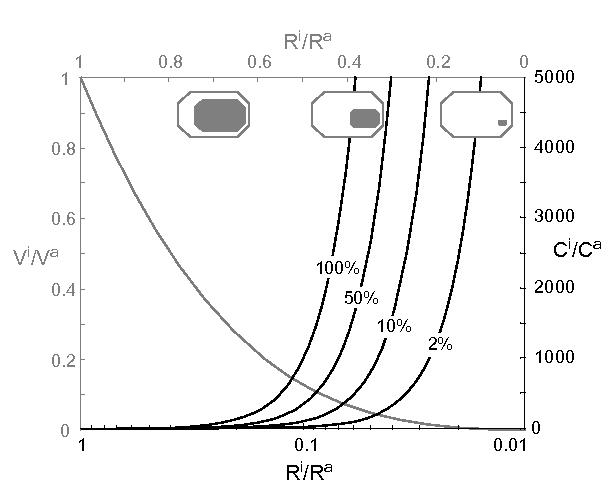
\includegraphics[width=0.6\textwidth]{viva2.jpg}
  \caption{
    Illustration  of the  ``blessings of  dimensionality''.   The gray
    line  shows, for  example, how  a tenfold  decrease of  the linear
    dimensions of a mineral inclusion (R$^i$ = length, width or height
    of the inclusion, R$^a$ =  length, width or height of the apatite)
    corresponds to  a thousandfold decrease  of its volume  (V$^i$ for
    the inclusion, V$^a$ for  the apatite) and $^4$He-production.  The
    black  lines show  the  U  or Th  concentrations  C$^i$ which  are
    required for the  inclusion to produce x\% of  the helium produced
    by a host apatite with concentration  C$^a$ (for x = 2, 10, 50 and
    100, respectively). Please note the different horizontal scale for
    the V$^i$/V$^a$ and the C$^i$/C$^a$ curves.}
  \label{fig:viva}
\end{figure}

\clearpage

\begin{center}
\uppercase{\section{The effect of $\alpha$-emitting mineral 
inclusions on $\alpha$-ejection corrections}}
\label{sec:math}
\end{center}

In the previous section, we  discussed the magnitude of the parentless
helium problem for small  mineral inclusions.  As will be demonstrated
later,  it is  possible to  avoid  this problem  altogether (even  for
relatively  large inclusions)  by  dissolving the  apatites and  their
mineral inclusions in aggressive acids such as HF.  However, this does
not  solve  a  second   problem,  caused  by  the  inhomogeneous  U-Th
concentrations associated with  mineral inclusions.  $\alpha$-decay of
U, Th and  their radioactive daughters is associated  with energies of
4-8  MeV (Farley  et al.,  1996).  $\alpha$-particles  with  such high
energies travel on average 20 $\mu$m in apatite before coming to rest.
Consider a  spherical apatite with  radius R and  an $\alpha$-emitting
nuclide located at a radial distance  X from its center.  Let S be the
$\alpha$-stopping  distance   (e.g.,  20  $\mu$m).   $\alpha$-emitting
nuclides  located  at a  distance  R-S$\leq$X$\leq$R  have a  non-zero
probability of ejecting an $\alpha$-particle outside the boundaries of
the  apatite  grain  (Figure  \ref{fig:FtivsXstar}).   For  any  given
spatial  distribution of  U  and Th,  it  is possible  to predict  the
fraction (1-F$_t$) of radiogenic  He lost by $\alpha$-ejection (Farley
et al.,  1996; Meesters and Dunai,  2002; Hourigan et  al.  2005).  In
most  cases, the  U-Th distribution  is not  known and  assumed  to be
uniform.  This assumption often constitutes the bulk of the analytical
(U-Th)/He  age uncertainty.  If  significant He  is produced  by small
mineral inclusions, the assumption of uniform composition is violated.
We  will  address  this  problem mathematically  for  spherical  grain
geometries.  The physical dimension  of the mineral inclusions will be
neglected,   i.e.   they   will   be  considered   point  sources   of
$\alpha$-particles, making the  He-retentivity of the inclusion itself
irrelevant.
\\

If  F$_t^a$ is  the $\alpha$-retention  fraction of  the  apatite, and
F$_t^i$ is  the fraction of  $\alpha$-particles that are  ejected from
the  inclusion   but  remain  inside  the  apatite,   then  the  total
$\alpha$-retention factor F$_t$ can be defined as:

\begin{equation}
  \label{eq:Ft}
  F_t = G F_t^i + (1-G) F_t^a
\end{equation}

where G  is the fraction of $\alpha$-decay activity ($\pi$) associated
with the mineral inclusion:

\begin{equation}
  \label{eq:G}
  G = \frac{\pi(inclusion)}{\pi(inclusion)+\pi(apatite)}
\end{equation}

\begin{equation}
  \label{eq:pi}
  \mbox{and~} \pi = 8^{238}\lambda[^{238}U] + 7^{235}\lambda[^{235}U] + 
        6^{232}\lambda[^{232}Th] + ^{147}\lambda[^{147}Sm] 
\end{equation}

with $^n\lambda$  the decay  constant and [n]  the number of  atoms or
moles of nuclide n (for n =  238, 235, 232 or 147). Note that equation
\ref{eq:pi} considers  He-production to be a linear  function of time,
which is  a good approximation  for relatively young samples  (t $\ll$
1/$^{n}\lambda$ $\forall$  n).  Our goal is to  derive the probability
distribution of  F$_t$.  To  achieve this goal,  we first  compute the
cumulative  distribution  function  (cdf)  of  the  $\alpha$-retention
factor F$_t^i$:

\begin{equation}
  \label{eq:CDFti}
cdf_{F_t^i}(f_t^i) \equiv Pr(F_t^i \leq f_t^i) = \begin{cases}
           \hfill 0 &\text{if} \quad (2-S/R)/4 > f_t^i \\
           \hfill 1 - cdf_{X^*}(x^*)
                  &\text{if} \quad (2-S/R)/4 \leq f_t^i < 1 \\
           \hfill 1 &\text{if} \quad f_t^i \geq 1 \\
         \end{cases}
\end{equation}

\begin{equation}
  \label{eq:cdfX}
\mbox{with~}  cdf_{X^*}(x^*) \equiv P(X^* \leq x^*) = \left(x^*\right)^3
\end{equation}

Where   X$^*$  is   the  nondimensional   radial   distance  X$^*$=X/R
corresponding to the $\alpha$-retention factor F$^i_t$.  cdf$_{F_t^i}$
can be computed because there  exists a unique mapping between F$_t^i$
and X$^*$  (Figure \ref{fig:FtivsXstar}),  derived from equation  1 of
Farley et al. (1996):

\begin{equation}
  \label{eq:FtvsXR}
  F_t^i\left(X^*\right) = 
  \frac{1-\left(X^*-\frac{S}{R}\right)^2}{4\frac{S}{R}X^*}
\end{equation}

\begin{equation}
  \label{eq:xRvsFt}
\mbox{and~}  X^*\left(F_t^i\right) = \left(\frac{S}{R}\right)\left(1-2F_t^i\right) +
             \sqrt{4\left(\frac{S}{R}\right)^2\left(F_t^i-1\right)F_t^i + 1}
\end{equation}

\begin{figure}[htbp]
  \centering
  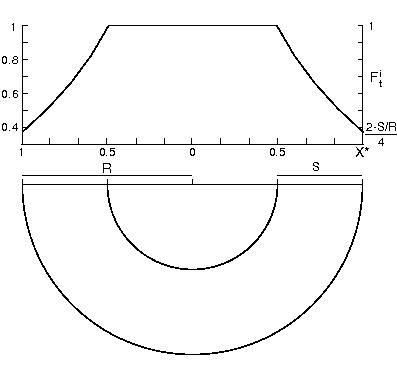
\includegraphics[width=0.5\textwidth]{FtivsXstar.jpg}
  \caption{Bottom: cross-section through the lower hemisphere of a spherical apatite with radius R.
    Top:  $\alpha$-retention factor  F$_t^i$ for  U-Th-bearing mineral
    inclusions as  a function  of the non-dimensional  radial distance
    X$^*$.  All  $^4$He produced by inclusions  located at X$^*<$1-S/R
    will  remain inside  the host  apatite  ($\Rightarrow$ F$_t^i$=1),
    with  S  the   $\alpha$-stopping  distance.   However,  inclusions
    located at X$^*>$1-S/R will eject a fraction (1-F$_t^i$) of helium
    outside the boundaries of the apatite.}
  \label{fig:FtivsXstar}
\end{figure}

The probability  density functions (pdfs) are then  easily obtained by
taking derivatives of the cdfs:

\begin{equation}
  \label{eq:PDFti}
  pdf_{F_t^i}(f_t^i) = \frac{d(cdf_{F_t^i}(f_t^i))}{d(f_t^i)}
\end{equation}

\begin{equation}
  \label{eq:PDFx*}
\mbox{and~}  pdf_{X^*}(x^*) = \frac{d(cdf_{X^*}(x^*))}{d(x^*)} = 3(x^*)^2
\end{equation}

Using  equations \ref{eq:PDFti} and  \ref{eq:PDFx*}, we  can calculate
$\bar{F_t^i}$,  the  expected  value  of  F$_t^i$  assuming  that  the
inclusions  have  a  spatially  uniform  distribution.   Here  we  use
``expected value'' in  the statistical sense of the  word, meaning the
average F$_t^i$ of  many apatites containing a few  inclusions, or the
average F$_t^i$ of a  few apatites containing many inclusions.  Thanks
to the  mapping between  F$_t^i$ and X$^*$  (equations \ref{eq:FtvsXR}
and  \ref{eq:xRvsFt} and  Figure  \ref{fig:FtivsXstar}), $\bar{F_t^i}$
can be  calculated either by integrating  over F$_t^i$ or  over X$^*$. 
Not surprisingly,  both approaches yield the same  result, which turns
out to be the analytical solution for F$_t^a$ under spherical geometry
calculated  by Farley  et al.  (1996) for  compositionally homogeneous
apatite:

\begin{equation}
  \label{eq:FtBar}
  \bar{F_t^i} = \int_{0}^{1} f_t^i ~ pdf_{F_t}(f_t^i) ~ df_t^i 
            = \int_0^1 F_t^i(x^*) ~ pdf_{X^*}(x^*) ~ dx^*
            = ... 
            = 1 - \frac{3}{4}\frac{S}{R} + \frac{1}{16}\left(\frac{S}{R}\right)^3
            = F_t^a
\end{equation}

The probability  distribution of  F$_t$ (equation \ref{eq:Ft})  can be
calculated  for any G  from the  probability distribution  for F$_t^i$
(equation  \ref{eq:PDFti}) and  the  expression for  F$_t^a$ given  by
Farley   et   al.    (1996)   and  equation   \ref{eq:FtBar}   (Figure
\ref{fig:CDFt}).  Although G is not known in most cases, our ignorance
about G can be quantified  by assigning a probability density function
pdf$_G$  to it.   Again,  to derive  the  probability distribution  of
F$_t$,  we   must  first   define  its  cumulative   density  function
cdf$_{F_t}$:

\begin{equation}
  \label{eq:CDFt}
  cdf_{F_t}(f_t) = \int_{0}^{1} cdf_{F_t^i}\left(\frac{f_t+(g-1)F_t^a}{g}\right) ~
                 pdf_G(g) ~ dg
\end{equation}

\begin{figure}[htbp]
  \centering
  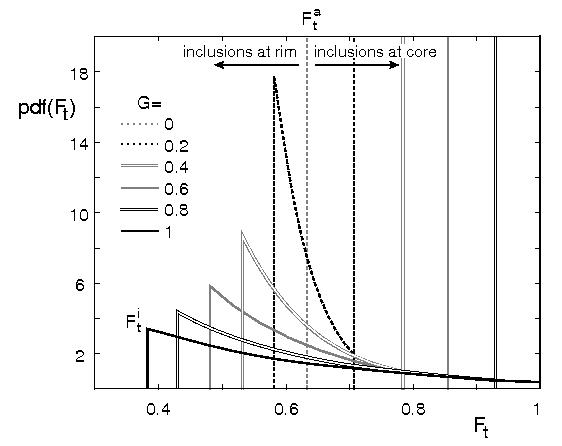
\includegraphics[width=0.7\textwidth]{pdFtG1.jpg}
  \caption{
    The expected spread of $\alpha$-retention factors F$_t$ for grains
    of a  single size  (S/R =  0.5) if the  inclusions are  located in
    different radial  positions within a spherical  apatite grain. The
    six curves correspond to inclusions of different $\alpha$-emitting
    activity  (G-value,  equation \ref{eq:G}).   More  helium will  be
    retained  from apatites  containing  an $\alpha$-emitting  mineral
    inclusion  at  their core  than  from  inclusion-free apatites  or
    apatites containing an inclusion near their rim.}
  \label{fig:CDFt}
\end{figure}


with cdf$_{F_t^i}(\cdot)$ as defined in equation \ref{eq:CDFti}, after
which pdf$_{F_t}$ is obtained by taking the derivative:

\begin{equation}
  \label{eq:PDFt}
  pdf_{F_t}(f_t) = \frac{d(cdf_{F_t}(f_t))}{d(f_t)}
\end{equation}

Figure  \ref{fig:PFt2D}  shows   pdf$_{F_t}$  for  a  uniform  pdf$_G$
distribution and  various S/R-values. The mode of  the distribution is
always  at   F$_t^a$,  with   heavy  tails,  especially   toward  high
$\alpha$-retentivities.  If  a ``normal'' $\alpha$-ejection correction
is made (F$_t  \equiv$ F$_t^a$) the most frequently  measured age will
be accurate, but some  other measurements will not. ``Undercorrected''
ages  will  generally  be  further  removed from  the  true  age  than
``overcorrected'' ages. It would  be relatively easy to compute F$_t$-
and corresponding  age-distributions for different,  and possibly more
realistic pdf$_G$s such as the logistic normal distribution.  However,
such an exercise is of limited interest because in reality, pdf$_G$ is
not known.  Nevertheless, the  main features of Figures \ref{fig:CDFt}
and  \ref{fig:PFt2D} are  robust:  the mean  value  of F$_t^i$  equals
F$_t^a$  and therefore  the  mean  value of  F$_t$  is independent  of
pdf$_G$.  The distribution of F$_t$ has a sharp mode at F$_t^a$, with
tails  towards lower  and  higher values (Figure \ref{fig:PFt2D}).\\

\begin{figure}[htbp]
  \centering
  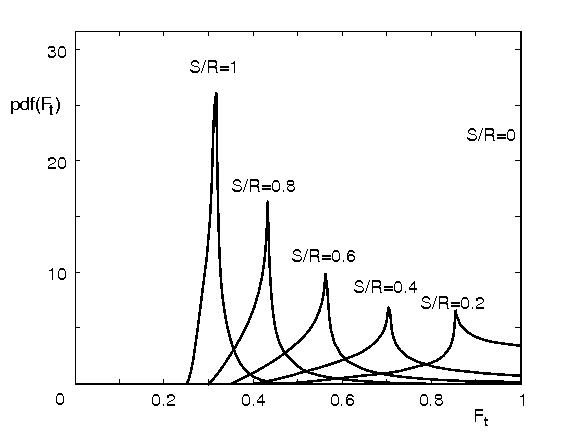
\includegraphics[width=0.7\textwidth]{pdFtUniformG.jpg}
  \caption{Probability density of the true $\alpha$-retention factor F$_t$
    for   uniform   G-distribution   ($pdf_G$(g)   dg   =   1/dg   for
    0$\leq$g$\leq$1) and various grain-sizes (S/R-values). Each of the
    curves  is  the  result  of  ``stacking''  the  curves  of  Figure
    \ref{fig:CDFt}.}
  \label{fig:PFt2D}
\end{figure}

Given the probability distribution of F$_t$ (equation \ref{eq:PDFt}), 
the standard deviation of F$_t$ can be calculated as:

\begin{equation}
  \label{eq:sigmaFt}
  \sigma(F_t) = \int_0^1 \left(f_t - \bar{F_t}\right)^2 pdf_{F_t}(f_t) ~ d(f_t)
\end{equation}

Where    $\bar{F_t}$   =    $F_t^a$    (equations   \ref{eq:Ft}    and
\ref{eq:FtBar}).  The  relative spread ($\sigma$($F_t$)/F$_t$)  of the
single grain $\alpha$-retention factor F$_t$ depends on the grain size
(Figure \ref{fig:sigmaFtvsSr}).   For very  small grains (S/R  $>$ 2),
the  spread  is  zero because  all  $^4$He  is  ejected (F$_t$  =  0),
irrespective  of the presence  or absence  of mineral  inclusions. For
very large grains (S/R $\approx$ 0), the spread of F$_t$ is also zero,
because all  $^4$He stays within  the apatite (F$_t$ $\approx$  1) and
the chance  that a mineral  inclusion is located within  the outermost
fraction S/R of such an apatite is negligible.  However, between these
two  extremes,  the  spread   of  the  $\alpha$-retention  factors  is
non-zero,   reaching   a  maximum   at   S/R   $\approx$  0.6,   where
$\sigma(F_t)$/F$_t$  $\approx$  0.2.   Please  note that  because  the
F$_t$-distribution    is     not    normally    distributed    (Figure
\ref{fig:sigmaFtvsSr}),  the  2$\sigma$-value  of  40\%  must  not  be
interpreted as the usual 95\% confidence interval.  However, by virtue
of  the   Central  Limit  Theorem,  the  average   of  n  single-grain
measurements  converges   to  a  normal   distribution  with  standard
deviation  $\sigma$(F$_t$)/$\sqrt{n}$.    For  example,  the  expected
2$\sigma$-spread  (corresponding  to a  95\%  confidence interval)  of
F$_t$-values for multi-grain packages containing n=10 grains each with
one inclusion,  or single grains with  n = 10 inclusions  is less than
12\%.  If S/R = 1/3 (e.g., S =  20 $\mu$m and R = 60 $\mu$m), then the
2$\sigma$  confidence  interval  for  F$_t$  is  $\sim$  10\%  (Figure
\ref{fig:sigmaFtvsSr}). These estimates  are conservative because they
assume that  all the U and  Th is contained in  the mineral inclusions
and that the host apatite itself contains  no U or Th.  If this is not
the case, then the spread of the multi-grain ages will be smaller.

\begin{figure}[htbp]
  \centering
  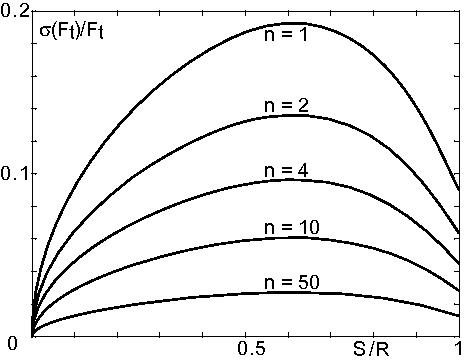
\includegraphics[width=0.5\textwidth]{sigmaFtvsSR.jpg}
  \caption{Relative spread of the $\alpha$-retention factors F$_t$ as a
    function of grain-size (S/R)  and for different multi-grain sample
    sizes (n  = 1, 2,  4, 10 and  50 grains, with  $\sigma$(F$_t|$n) =
    $\sigma$(F$_t|$1)/$\sqrt{n}$).}
  \label{fig:sigmaFtvsSr}
\end{figure}

\clearpage

%\begin{center}
\uppercase{
\section{The effect of $\alpha$-emitting mineral 
inclusions on closure temperatures}
}
\label{sec:Tc}
%\end{center}

Besides    complicating   the   $\alpha$-ejection    correction,   the
inhomogeneous U-Th-distribution inherent to inclusion-bearing apatites
also affects  the diffusive  behavior of the  helium. This  problem is
well studied  in the case  of concentrically zoned  spherical crystals
(Meesters  and Dunai,  2002b).  The  ``closure  temperature'' (defined
below) of the (U-Th)/He system  depends on the spatial distribution of
the  helium.   This does  not  constitute  a  significant problem  for
relatively rapidly cooled rocks (e.g.  $>$ 10 $^o$C/Ma for rocks older
than $\sim$10  Ma).  However, for  slowly cooled rocks, the  effect of
mineral  inclusions  on  helium  diffusion  might  induce  significant
scatter in the apparent ages, depending on the spatial distribution of
the   inclusions  and   their   relative  $\alpha$-emitting   activity
(G-factor,  equation  \ref{eq:G}),  which  are  nearly  impossible  to
measure.  To  get a  handle on the  significance of this  effect, this
section  will consider  the  ``worst case  scenario''  of a  spherical
U-Th-free apatite  containing an $\alpha$-emitting  micro-inclusion at
its  core  or  rim.  Such  a  grain  should  have the  most  different
diffusive behavior  compared to the default case  of an inclusion-free
apatite containing a homogeneous U-Th-distribution.
\\

Before  proceeding with  the  analysis,  it is  useful  to recall  the
definition  of  ``closure   temperature''  by  Dodson  (1973).   First
consider the case of  isothermal diffusion for a simple geochronometer
defined by  one radioactive  parent P (e.g.,  $^{40}$K) decaying  to a
radiogenic daughter  D (e.g.,  $^{40}$Ar).  At high  temperatures, the
radiogenic  daughter escapes  from mineral  grains  as soon  as it  is
formed whereas  at low temperatures, thermally  activated diffusion is
negligible and the daughter products are quantitatively retained.  Now
consider the case of  monotonic cooling.  In the high-temperature part
of the  cooling-curve, the  D/P-ratio stays zero.   Under transitional
temperatures, the  D/P-ratio increases at  a rate that  increases with
time.  Finally, at low temperatures, D/P increases linearly with time.
The apparent  age is the time  intercept of the linear  section of the
D/P vs time  curve.  This age corresponds to  a particular temperature
in the  cooling history, the so-called ``closure  temperature'' T$_c$. 
If the cooling curve is linear  in the temperature T, then the closure
temperature (T$_c$) is the temperature intercept of the linear section
of the T vs D/P curve  (Figure \ref{fig:Tt}).  If the cooling curve is
linear  in 1/T,  then T$_c$  can be  calculated  analytically (Dodson,
1973).   Things are a  little more  complicated for  (U-Th)/He because
there are not one but three radioactive parents ($^{238}$U, $^{235}$U,
and  $^{232}$Th)  with different  half-lives,  causing their  relative
contributions  to change with  time.  However,  the helium  content of
young  rocks  does  increase  linearly   with  time  to  a  very  good
approximation  (t  $\approx$  [He]/$\pi$  with  $\pi$  as  defined  in
equation \ref{eq:pi}). Therefore,  the closure temperature concept can
also  be  used  for  (U-Th)/He.   Because we  are  interested  in  the
relationship between  mineral inclusions and cooling  rate (dT/dt), we
will assume  linear cooling  (dT/dt = constant  with t).  We  will not
calculate  T$_c$ using  Dodson's approximate  analytical  solution (an
exact solution is only possible if T $\propto$ 1/t).  Instead, we will
calculate T$_c$ numerically using the DECOMP program of Bikker,
Meesters and Dunai (Dunai, 2005).\\

As  said  before,  in  the   case  of  linear  cooling  T$_c$  is  the
temperature-intercept of a  curve plotting temperature versus apparent
(U-Th)/He age  (Figure \ref{fig:Tt}).  Thanks to a  combination of the
``superposition principle''  (Meesters and Dunai, 2002a \&  b) and the
spherical  symmetry,  a  concentrated $\alpha$-emitting  inclusion  is
mathematically  equivalent  to a  thin  spherical  shell  at the  same
distance of  the rim  (A.G.C.A. Meesters, written  communication, July
2006).  A spherical shell of  a certain U-Th concentration produces as
much He as a half-shell with twice, or a quarter-shell with four times
this U-Th  concentration.  By  induction it follows  that a  U-Th rich
spherical   shell  is   equivalent  to   a  point   source   of  equal
$\alpha$-emitting activity located at the  same distance from the rim. 
Therefore,  individual   inclusions  can  be   adequately  modeled  as
spherical shells in  DECOMP.  The ``worst case scenario''  of a single
$\alpha$-emitting micro-inclusion located in the center of a U-Th-free
apatite was modeled  in DECOMP by a spherical zone  of 1 $\mu$m radius
containing all the U and Th, contained in a much larger spherical host
apatite  (e.g., R  = 60  $\mu$m  in Figure  \ref{fig:Tt}), whereas  an
inclusion  located on  the rim  of such  an apatite  was modeled  by a
spherical shell  of 1 $\mu$m thickness.  Given  a user-defined cooling
curve (10 $^o$C/Ma for Figure \ref{fig:Tt}), DECOMP forward-models the
apparent  age  through time  using  an eigenmode-decomposition  method
(Meesters  and  Dunai,  2002a \&  b).   In  this  paper, we  used  100
eigenmodes.   The apparent  age increases  linearly with  time  in the
lower   temperature  part   of  the   linear  cooling   model  (Figure
\ref{fig:Tt}).   As expected,  the  linear section  of  the T-t  curve
begins at higher temperatures  for the apatite containing an inclusion
at its core than  for inclusion-free apatite.  Intuitively, this makes
sense  because the  helium  produced by  the  inclusion must  ``travel
further'' before  reaching the edge  of the apatite.  The  opposite is
true for apatites with an inclusion on their rim.
\\

The  closure  temperature   calculation  was  repeated  for  different
grain-sizes (40 $\mu$m  $\leq$ R $\leq$ 130 $\mu$m)  and cooling rates
(10 $^o$C/Ma  and 1 $^o$C/Ma)  (Figure \ref{fig:Tc}).  In  the ``worst
case scenario''  of an inclusion-bearing apatite, T$_c$  is 5-10 $^o$C
higher or  lower than in the  absence of inclusions.  This  is a small
effect in several respects.  First of all, the ``worst case scenario''
used for the  calculations of Figure \ref{fig:Tc} is  very unlikely to
ever  occur  in  nature.   As explained  in  Section  \ref{sec:micro},
mineral inclusions never  contain 100\% of $\alpha$-emitting activity,
because their relative volume is small and the U-Th content of apatite
is  never zero.   Consider the  more realistic  scenario of  a mineral
inclusion contributing 50\% of the total helium (G = 0.5).  Because of
the superposition principle, such an inclusion will change the closure
temperature by  only 2.5-5  $^o$C.  The effects  of grain  size (15-20
$^o$C  difference   in  T$_c$  between  40  and   130  $\mu$m,  Figure
\ref{fig:Tc}) and  cooling rate ($\sim$  15 $^o$C difference  in T$_c$
between  1 and  10 K/Ma,  Figure  \ref{fig:Tc}) are  greater than  the
inclusion-effect.  Therefore, it should  also be possible to apply the
HF-dissolution  method  to  slowly  cooled  rocks.   However,  several
studies have reported irreproducible apatite (U-Th)/He ages for slowly
cooled  terranes (Fitzgerald et  al., 2006)  and (U-Th)/He  ages older
than apatite  fission track  ages (Soderlund et  al., 2005;  Green and
Duddy,   2006).    Therefore,  the   next   section   will  test   the
HF-dissolution method on rapidly cooled rocks.

\begin{figure}[htbp]
  \centering
  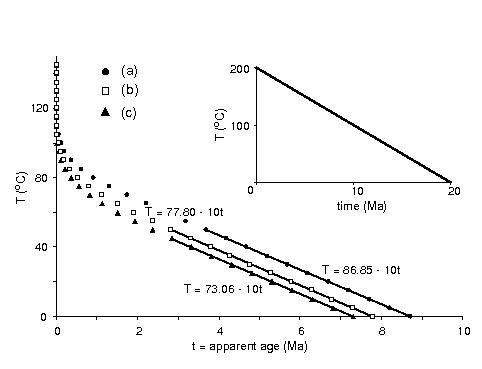
\includegraphics[width=0.7\textwidth]{Tt10KMa60um2.jpg}
  \caption{
    Closure temperature  (T$_c$) calculation using  the DECOMP program
    (Dunai,  2005).  The  inset shows  a linear  cooling curve  with a
    cooling rate of 10$^o$C/Ma.  In this case, the closure temperature
    can be  defined as  the y-intercept of  the linear section  of the
    temperature  vs.  age  curve (Dodson,  1973).  (a)  ``worst case''
    scenario of  a U-Th-free apatite with a  U-Th-bearing inclusion at
    its  center  (closure  temperature   T$_c$  =  86.85  $^o$C);  (b)
    inclusionless apatite of uniform U, Th concentration (T$_c$ = 77.8
    $^o$C).  (c) ``worst case'' scenario of a U-Th-free apatite with a
    U-Th-bearing inclusion at its edge (T$_c$ = 73.06).  Radius of the
    host  apatite  = 60  $\mu$m,  $\alpha$-stopping  distance  S =  20
    $\mu$m.}
  \label{fig:Tt}
\end{figure}

\begin{figure}[htbp]
  \centering 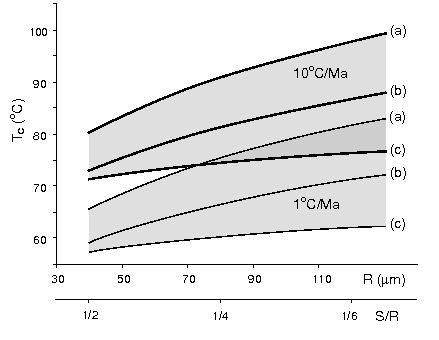
\includegraphics[width=0.6\textwidth]{Tc2.jpg}
  \caption{
    Repeating  the  numerical experiment  of  Figure \ref{fig:Tt}  for
    different  grain sizes  and  cooling rates,  this  plot shows  the
    evolution of closure  temperature T$_c$ with grain size,  (a \& c)
    with  and (b) without  the presence  of a  mineral inclusion  in a
    spherical  apatite with  radius R,  for relatively  rapidly cooled
    (10$^o$C/Ma, thick lines) and  very slowly cooled (1$^o$C/Ma, thin
    lines)  rocks.  (a),  (b)  and   (c)  are  as  defined  in  Figure
    \ref{fig:Tt}.}
  \label{fig:Tc}
\end{figure}

\clearpage

%\begin{center}
\uppercase{
\section{Application to inclusion-rich apatites from Naxos, Greece}
}
\label{sec:nax}
%\end{center}

From the  archive of apatite fission-track  samples at ETH-Z\"{u}rich,
we  chose a  sample that  was both  rapidly cooled  and full  of large
mineral inclusions.  The sample,  NAX-3, comes from the migmatite core
on the eastern side of Naxos.  In fact, apatites from NAX-3 contain so
many inclusions that  it was quite challenging to  date them using the
fission-track  method.  Due  to the  U bearing  inclusions  which form
``stars''   on  the   mica   solid  state   track  recorders   (Figure
\ref{fig:FTmount&print}),  clear grains had  to be  chosen with  care. 
Nevertheless,  a fission-track age  of 9.5  $\pm$ 1.8  (2$\sigma$) was
measured  using the  $\zeta$  (zeta) calibration  method (Hurford  and
Green, 1983) (Figure  \ref{fig:NAX3radial}.a).  The U-concentration of
the apatites was determined to be $\sim$20 ppm.  Two additional zircon
fission-track  ages  were  recorded  by  Zingg (2004)  from  the  same
migmatite  at  9.7  $\pm$  1.0  and  10.6  $\pm$  2.0  Ma  (2$\sigma$)
confirming the rapid cooling.
\\

\begin{figure}[htbp]
  \centering
a. 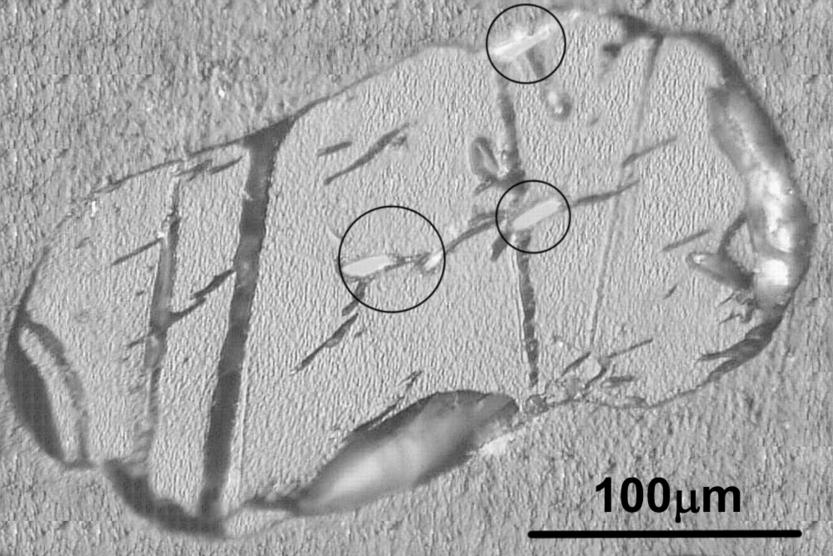
\includegraphics[height=4cm]{FTmount1gray.jpg}
b. 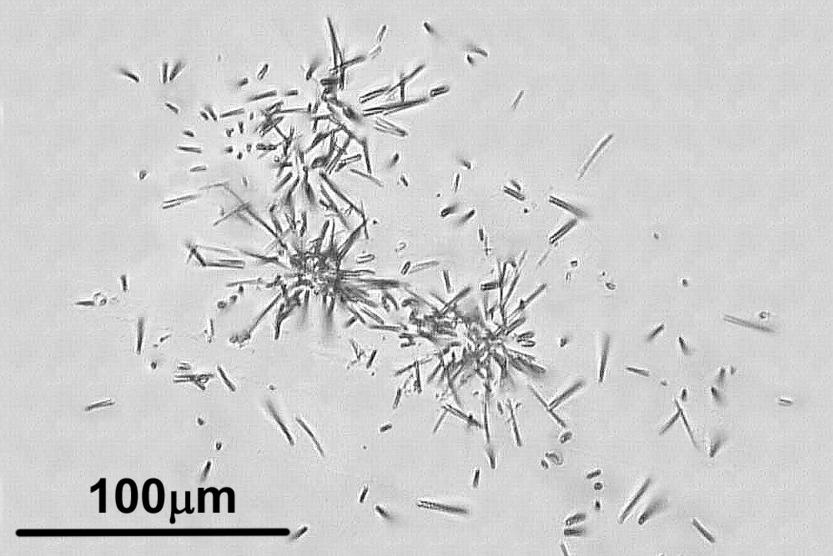
\includegraphics[height=4cm]{FTprint1gray.jpg}
  \caption{
a. NAX-3 apatite with inclusions (encircled) mounted in epoxy; b.  The
mica-print  of the  same apatite  shows ``stars''  of  induced fission
tracks, indicating  that the inclusions have a  higher U concentration
than the surrounding apatite. The  inclusions have a smaller effect on
the (U-Th)/He  age than the  track density of the  ``stars'' suggests,
because the  fission-track map  is a two-dimensional  cross-section of
the   apatite,   whereas  the   (U-Th)/He   age   is   based  on   the
three-dimensional,  volumetric  U-Th-He content  of  the apatite.   To
estimate  the effect  of these  inclusions on  the (U-Th)/He  age, and
assuming  that the  inclusions  are 10\%  of  the length  of the  host
apatite, one  would effectively have  to divide the number  of fission
tracks in the ``stars'' by a factor of ten.}
  \label{fig:FTmount&print}
\end{figure}

\begin{figure}[htbp]
  \centering
a. 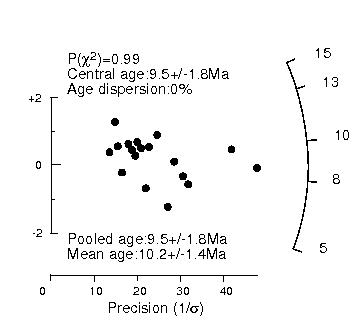
\includegraphics[width=.45\textwidth]{NAX3radial.jpg}
b. 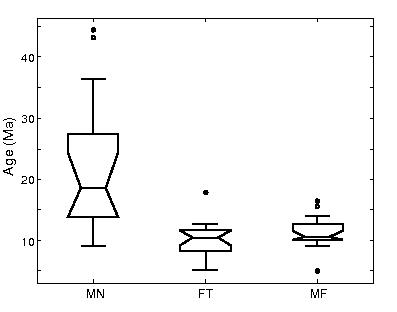
\includegraphics[width=.45\textwidth]{boxplots.jpg}
  \caption{
    a.  Apatite fission-track radial plot (Galbraith, 1990) for NAX-3.
    b.  Box-plots  (McGill et al.,  1978) for (U-Th)/He data  of NAX-3
    apatites dated using two acid dissolution treatments: HNO$_3$ (MN,
    left side  of the figure) and HF  (MF, right side of  the figure). 
    The middle box plot (``FT'') shows the fission track data.}
  \label{fig:NAX3radial}
\end{figure}

Inspection  under a  binocular microscope  (200$\times$ magnification)
revealed that most  inclusions are zircon, based on  crystal shape and
reflectance (Figure  \ref{fig:W1}). Zircons are the  ``right'' kind of
inclusion for the present study, because they are particularly hard to
dissolve.   After measuring their  size under  the microscope  for the
calculation of F$_t^a$, the apatites were packed in Pt foil tubes. Two
batches  of  grains were  prepared:  26  single  grain packets  and  7
multi-grain packets with  inclusion-bearing apatites (labels beginning
with ``M'' in Table \ref{tab:UThHe}) and four multi-grain packets with
inclusion-free  apatites   (labels  beginning  with   ``Z''  in  Table
\ref{tab:UThHe}).

\begin{figure}[htbp]
  \centering     a.     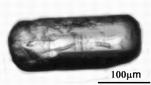
\includegraphics[width=.27\textwidth]{w1b.jpg}
b.                       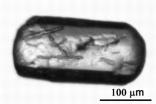
\includegraphics[width=.27\textwidth]{w1a.jpg}
c. 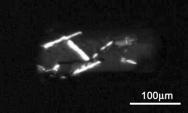
\includegraphics[width=.3\textwidth]{w1c.jpg}
  \caption{
    Example of a  NAX-3 grain (MF1) with large  zircon inclusions. The
    dimensions  of  the apatite  are  262  $\times$  127 $\times$  106
    $\mu$m. Pictures a and b show the grain under plain light, whereas
    picture c was taken under crossed polarizers.}
  \label{fig:W1}
\end{figure}

Helium contained  in the  apatites was extracted  during 3  minutes of
laser heating  under ultra-high vacuum (10$^{-8}$ Torr),  using a 1064
nm  wavelength  Nd-YAG laser.   Re-extraction  experiments yielded  no
detectable  helium,  indicating  complete  degassing.   Following  its
release from the samples, the gas was cleaned in a liquid N$_2$ cooled
activated charcoal cold finger and Ti/Zr and Al/Zr getters. $^4$He was
measured by  peak height calibration to  a bottle of  known amounts of
$^4$He  in  a   custom-built  sector-type  mass  spectrometer.   After
He-analysis,  the  Pt  packets  were  recovered from  the  laser  pan,
partially  opened under  the  binocular microscope,  and dropped  into
teflon bombs. Because Pt dissolves  in HF and forms PtAr interferences
in the ICP-MS plasma (Reiners, 2005), we had to recover the Pt packets
before  HF treatment.   Using Nb  foil  envelopes would  have been  an
alternative solution  (Reiners, 2005).  In  nearly half of  the cases,
dropping the  samples into the  teflon bombs caused the  apatite(s) to
fall  out  of  their  partially  opened  packet.   These  grains  were
specifically  selected  for  later  HF-treatment  in  order  to  avoid
complications of PtAr interferences.   First however, all samples were
spiked  with   $\sim$50  fmol  of  $^{233}$U  and   $\sim$20  fmol  of
$^{229}$Th.    $\sim$1   ml    of   concentrated   and   high   purity
quartz-distilled  HNO$_3$  was  added   to  all  the  samples.   After
digestion on a hot plate ($\sim$150$^o$C) for one day, the HNO$_3$ was
dried down  for the inclusion-free  and half of  the inclusion-bearing
samples, and $\sim$1 ml of 6\%HNO$_3$-0.8\%HF solution was added.  For
these  samples  (labels beginning  with  ``MN''  and  ``ZN'' in  Table
\ref{tab:UThHe}), this  was the  final sample preparation  step before
the U-Th measurement.  For  the remaining 19 inclusion-bearing samples
(labels  beginning with  ``MF'' in  Table \ref{tab:UThHe}),  the empty
Pt-packets were  recovered from the teflon vials  prior to evaporation
of  the   concentrated  HNO$_3$.    After  dry-down,  $\sim$1   ml  of
concentrated,  high  purity  Teflon-distilled  HF was  added  and  the
samples were bombed in  an oven at 200$^o$C for 24 hours  and on a hot
plate at $\sim$240$^o$C for an  additional 48 hours. $\sim$ 100 $\mu$l
of  concentrated HNO$_3$  was added  to  the HF  for samples  MF16-19,
following  a  suggestion of  P.  Reiners  (written communication,  May
2006).  The HF was dried down  and the samples re-bombed in $\sim$1 ml
concentrated HCl  at $\sim$200$^o$C for 24 hours  to dissolve fluoride
salts  that may  have formed  during  HF evaporation.   After a  final
dry-down,  $\sim$1 ml  6\%HNO$_3$-0.8\%HF solution  was added  and the
samples were ready for  ICP-MS analysis.  This combined HNO$_3$-HF-HCl
treatment is tailored to dissolve larger crystals for zircon (U-Th)/He
dating (Reiners,  2005).  However,  zircons inclusions in  apatite are
generally  much smaller, and  a less  aggressive (e.g.,  shorter, less
hot) procedure
might also be suitable.\\

$^{229}$Th,  $^{232}$Th,  $^{233}$U,  $^{238}$U (and  $^{235}$U)  were
measured  in  low  mass  resolution on  a  single-collector  ICP-SF-MS
(Element2, Thermo Electron  Corporation, Bremen, Germany). The results
are summarized in Table  \ref{tab:UThHe}.  Immediate inspection of the
data  reveals that the  spread of  the zircon  inclusion-bearing grain
ages  is much larger  for the  HNO$_3$ treated  grains than  for those
treated with HF (Figure \ref{fig:NAX3radial}.b).  The former are up to
45 Ma old,  whereas the latter cluster more tightly  and are closer to
the fission-track age.  Using  the grain dimensions that were measured
for  the $\alpha$-ejection correction  as an  estimate of  mass yields
median  U and  Th concentrations  of $\sim$5  and $\sim$10ppm  for the
HNO$_3$-treated  grains, whereas the  U and  Th concentrations  of the
HF-treated grains was $\sim$6  and $\sim$14ppm respectively, closer to
the  fission track estimate  ($\sim$19ppm).  10  of the  14 HF-treated
single  grain samples are  between 9  and 13  Ma, consistent  with the
sharp mode  of Figure \ref{fig:PFt2D}.   As discussed in  the previous
section, the average age of multiple inclusion-bearing apatites should
be an  accurate estimate of the  true age. To compare  and combine the
single  grain  measurements  with  the  multi-grain  measurements,  we
introduce a ``pooled (U-Th)/He  age'', which effectively is a weighted
mean  age  obtained by  adding  the U  and  Th  of several  individual
analyses,    as    well   as    their    He-content   (weighted    for
$\alpha$-ejection), and calculating  a synthetic multi-grain age.  The
pooled age of the HNO$_3$-treated inclusion-bearing grains is 22.6 Ma,
whereas the  HF-treated pooled age is  10.9 Ma, which  is identical to
the pooled (U-Th)/He age of  the four inclusion-free apatite analyses. 
Note that the  (U-Th)/He age of one of  these four inclusion-free ages
is  nearly twice  as  old as  the  other three.   Because  we have  no
indication as to what is the cause of this, we chose not to reject the
measurement.   However,  if  the   measurement  is  removed  as  being
unrepresentative  the resulting  age is  9.2  Ma.  Fitzgerald  et al.  
(2006) also observed  single grain ages that were  several times older
than  ``normal''.   Perhaps one  of  the  factors  discussed by  these
authors is responsible  for this, or a yet  unknown complication is at
work.   As discussed  in Section  \ref{sec:math} and  shown  in Figure
\ref{fig:sigmaFtvsSr},  the spread  of HF-treated  multi-grain samples
should  be less  than that  of the  single grain  ages.   The relative
2$\sigma$-spread   of  multi-grain   packages   each  containing   ten
inclusion-bearing grains of 100 $\mu$m width (equivalent to S/R $\sim$
0.2) should be  less than $\sim$ 8 \%  (Figure \ref{fig:sigmaFtvsSr}). 
This  is  confirmed by  the  five  multi-grain  measurements of  Table
\ref{tab:UThHe} (MF15-19), which have a 2$\sigma$-spread of just 5\%.

\begin{table}[here]
%\begin{small}
  \centering
% Table generated by Excel2LaTeX from sheet '(U-Th)He'
\begin{tabular}{rrlllllllll}
    sample & \# grains &  Th  &  2$\sigma$ &  U   &  2$\sigma$ & He   &  2$\sigma$ &  F$_t^a$ & age  &  2$\sigma$ \\
   ~   &  & [fmol] & & [fmol] & & [fmol] & & & [Ma] & ~  \\
\hline
\hline
  MN1 & 1 & 104 & 4 & 81 & 2 & 3.96 & 0.14 & 0.66 & 44.5 & 9.3 \\
  MN2 & 1 & 550 & 19 & 2041 & 50 & 22.87 & 0.35 & 0.85 & 9.6 & 0.7 \\
  MN3 & 1 & 201 & 7 & 493 & 12 & 11.07 & 0.21 & 0.79 & 20.1 & 2.2 \\
  MN4 & 1 & 173 & 6 & 283 & 7 & 3.89 & 0.15 & 0.75 & 12.5 & 1.8 \\
  MN5 & 1 & 119 & 3 & 117 & 3 & 5.51 & 0.15 & 0.68 & 43.2 & 8.1 \\
  MN6 & 1 & 172 & 7 & 428 & 14 & 8.74 & 0.17 & 0.75 & 19.5 & 2.7 \\
  MN7 & 1 & 185 & 7 & 371 & 7 & 5.90 & 0.16 & 0.74 & 15.1 & 2.2 \\
  MN8 & 1 & 160 & 8 & 89 & 3 & 0.84 & 0.12 & 0.58 & 9.0 & 2.9 \\
  MN9 & 1 & 249 & 7 & 588 & 11 & 11.51 & 0.22 & 0.78 & 17.8 & 2.0 \\
 MN10 & 1 & 365 & 11 & 725 & 19 & 11.56 & 0.22 & 0.81 & 13.7 & 1.3 \\
 MN11 & 1 & 144 & 5 & 113 & 2 & 1.93 & 0.13 & 0.64 & 16.1 & 3.8 \\
 MN12 & 1 & 90 & 18 & 285 & 58 & 6.17 & 0.08 & 0.84 & 20.6 & 4.6 \\
 MN13 & 8 & 660 & 23 & 2358 & 73 & 93.39 & 1.38 & 0.79 & 36.5 & 4.0 \\
 MN14 & 10 & 2169 & 451 & 2710 & 554 & 91.60 & 0.28 & 0.85 & 27.5 & 5.3 \\
\hline
MN (pooled) & 30 & 5342 & 452 & 10682 & 565 &  345.32 & 1.55 & & 22.6 & 1.1 \\
\hline
\hline
  MF1 & 1 & 451 & 14 & 588 & 14 & 9.57 & 0.17 & 0.77 & 14.0 & 1.8 \\
  MF2 & 1 & 628 & 22 & 874 & 15 & 9.75 & 0.18 & 0.74 & 10.1 & 1.5 \\
  MF3 & 1 & 768 & 25 & 185 & 4 & 1.74 & 0.13 & 0.76 & 5.0 & 0.7 \\
  MF4 & 1 & 156 & 5 & 294 & 7 & 4.27 & 0.14 & 0.78 & 12.9 & 1.5 \\
  MF5 & 1 & 260 & 9 & 596 & 15 & 6.97 & 0.21 & 0.80 & 10.4 & 1.1 \\
  MF6 & 1 & 370 & 14 & 645 & 17 & 6.91 & 0.18 & 0.73 & 10.1 & 1.5 \\
  MF7 & 1 & 374 & 10 & 867 & 18 & 10.64 & 0.22 & 0.85 & 10.2 & 0.7 \\
  MF8 & 1 & 163 & 6 & 222 & 5 & 2.02 & 0.13 & 0.65 & 9.3 & 2.1 \\
  MF9 & 1 & 136 & 4 & 226 & 5 & 2.36 & 0.13 & 0.79 & 9.1 & 1.1 \\
  MF10 & 1 & 130 & 4 & 131 & 4 & 2.00 & 0.13 & 0.59 & 16.4 & 4.7 \\
  MF11 & 1 & 204 & 9 & 357 & 14 & 6.42 & 0.16 & 0.79 & 15.6 & 1.8 \\
 MF12 & 1 & 126 & 5 & 107 & 3 & 1.01 & 0.12 & 0.63 & 9.2 & 2.4 \\
 MF13 & 1 & 126 & 26 & 688 & 142 & 9.01 & 0.10 & 0.81 & 12.1 & 2.6 \\
 MF14 & 1 & 278 & 58 & 1013 & 212 & 11.75 & 0.10 & 0.86 & 10.6 & 2.3 \\
 MF15 & 10 & 27525 & 2179 & 5140 & 234 &  121.41 & 1.82 & 0.74 & 11.1 & 1.6 \\
 MF16 & 10 & 2557 & 523 & 7454 & 1525 & 84.64 & 0.22 & 0.85 & 10.1 & 2.1 \\
 MF17 & 10 & 1986 & 406 & 5610 & 1146 & 76.81 & 0.21 & 0.85 & 12.4 & 2.6 \\
 MF18 & 10 & 1327 & 274 & 3892 & 806 & 54.45 & 0.30 & 0.83 & 13.3 & 3.0 \\
 MF19 & 11 & 919 & 190 & 2578 & 533 & 28.01 & 0.17 & 0.79 & 10.6 & 2.5 \\
\hline
MF (pooled) & 64 & 38487 & 2303 & 31467 & 2166 &  563.09 & 1.96 & & 10.9 & 0.6 \\
\hline
\hline
  ZN1 & 5 & 151 & 7 & 182 & 8 & 4.20 & 0.14 & 0.70 & 21.5 & 3.9 \\
  ZN2 & 3 & 164 & 6 & 262 & 8 & 2.20 & 0.12 & 0.69 & 8.2 & 1.5 \\
  ZN3 & 1 & 175 & 5 & 515 & 13 & 4.93 & 0.14 & 0.81 & 8.5 & 0.8 \\
  ZN4 & 4 & 175 & 6 & 454 & 11 & 4.61 & 0.15 & 0.68 & 10.7 & 2.0 \\
\hline
ZN (pooled) & 13 & 666 & 12 & 1414 & 21 & 21.99 & 0.28 & & 10.9 & 0.2 \\
\hline
\hline
\end{tabular}
%\begin{small} 
\caption{
(U-Th)/He data for: MN = grains with inclusions, dissolved in HNO$_3$;
MF = grains with inclusions, dissolved in HF; ZN = grain without
inclusions, dissolved in HNO$_ 3$. The $^4$He values for the ``pooled
ages'' have been adjusted for $\alpha$-ejection of the component
grains. Age uncertainty includes an arbitrary 20\% uncertainty on
(1-F$_t^a$). The pooled 2$\sigma$-uncertainties only incorporate the
analytical precision and do not reflect the spread of the component
single-grain measurements.}
 \label{tab:UThHe}
\end{table}

\clearpage

\begin{center}
\uppercase{\section{Discussion}}\label{sec:discussion}
\end{center}

Simple  dimensional considerations  indicate that  single uranium-rich
inclusions less than a few percent  of the length, width and height of
the  host apatite  are unlikely  to contribute  substantial radiogenic
helium.   For  larger inclusions  or  multiple  small inclusions,  the
parentless helium  problem can be partially solved  by more aggressive
acid  dissolution  procedures.   Under  the  assumption  of  uniformly
distributed  mineral inclusions,  the  average (U-Th)/He  age of  many
inclusion-rich  apatites  that  have  undergone such  a  treatment  is
accurate. Please note that the assumption of a random distribution can
more easily  be verified  in the presence  of large  inclusions (e.g.,
Figure  \ref{fig:W1}) than for  micro-inclusions or  a compositionally
zoned  apatite.  Grain-selection  is significantly  faster  and easier
without the  restriction to inclusion-free grains.   For some samples,
it is  nearly impossible to  find inclusion-free grains.   Further, by
broadening the search to  include inclusion-bearing grains, it is much
easier to  find large,  euhedral apatites, requiring  relatively small
$\alpha$-ejection corrections. Additionally, the presence of U-Th rich
inclusions may be an advantage  for dating young rapidly cooled rocks. 
Multi-grain  measurements of  inclusion-bearing  apatites combine  the
best of two worlds. They have the high U, Th and He content of zircon,
but  the diffusive behavior  and uniquely  low closure  temperature of
apatite. This  is similar to the  idea behind the  work of Min et  al. 
(2006), who dated volcanic olivine  and pyroxene using the He produced
by  the $\alpha$-emitting  inclusions  contained within  them. On  the
other  hand,   dissolving  U-Th  rich  inclusions   also  causes  some
complications, particularly for single-grain dating. The
probability distribution of single grain ages has heavy tails.\\

The revised methodology has  applications to all rock-types which have
inclusion-bearing  apatites.  However, in  most  studies,  only a  few
grains are usually dated and it is often possible to find two or three
suitable clear crystals. For  detrital source studies however, this is
not the case because in such studies many more grains are necessary to
characterize  the   population.  The  difficulty   of  finding  enough
inclusion-free  grains that represent  a realistic  and representative
cross section  of the populations can  only be made  by also including
some  of the  inclusion-bearing  apatites. Although  the precision  of
single  grain (U-Th)/He  ages on  inclusion-bearing apatites  is worse
than  the precision of  inclusion-free apatite  (U-Th)/He ages,  it is
comparable to or better than the precision of detrital apatite fission
track ages. Thus we recommend  that for detrital studies using apatite
analysis the more aggressive dissolution method is used routinely.
\\

\newpage

{\it Acknowledgments} This manuscript benefited from input from Rainer
Wieler and comments from Peter Reiners and two anonymous reviewers. 
Pieter Vermeesch is financially supported by a Marie Curie Fellowship
of the European Union (CRONUS-EU network).

\section*{References}

\begin{description}
 
\item Carter, T. J., Kohn, B. P., Foster, D. A., and Gleadow, J. W. 
 (2004) How the Harcuvar Mountains metamorphic core complex became
 cool: Evidence from apatite (U-Th)/He thermochronometry. Geology
 (32) 985-988.

\item Deer, W.A., Howie, R.A., and Zussman, J. (1992) An Introduction
 to the Rock-Forming Minerals, 2nd edition. Longman Scientific and
 Technical Press, 696 pp.
 
\item Dodson, M.H. (1973) Closure temperature in cooling
 geochronological and petrological systems. Contrib. Mineral. 
 Petrol., (40) 259-274.

\item Dunai, T. J. (2005), Forward modeling and the interpretation 
of (U-Th)/He ages. Reviews in Mineralogy and Geochemistry, Vol. 58 
(ed. P. W. Reiners and T. A. Ehlers), pp. 259-247.

\item Ehlers T. A. and Farley K. A. (2003) Apatite (U-Th)/He
Thermochronometry: methods and applications to problems in tectonics
and surface processes. Earth and Planetary Science Letters 206(1-14).

\item Farley K. A., Wolf R. A., and Silver L. T. (1996) The effects of
long alpha-stopping distances on (U-Th)/He ages. Geochimica et
Cosmochimica Acta 60(21), 4223-4229.

\item Farley K. A. and Stockli D. (2002) (U-Th)/He Dating of
Phosphates: Apatite, Monazite, and Xenotime. In Phosphates, Reviews
in Mineralogy and Geochemistry, Vol. 15 (ed. M. Kohn, J. Rakovan, and
J. M. Hughes), pp. 559-578.

\item Farley, K.A. (2002) (U-Th)/He dating: Techniques, calibrations,
and applications. In Noble Gases in Geochemistry and Cosmochemistry,
Reviews in Mineralogy and Geochemistry, Vol. 47 (ed. Porcelli, D.P.,
Ballentine, C.J., and Wieler, R.), pp. 819-844.

\item Fitzgerald P. G., Baldwin S. L., Webb L. E., and O'Sullivan
P. B. (2006) Interpretation of (U-Th)/He single grain ages from slowly
cooled crustal terranes: A case study from the Transantarctic
Mountains of southern Victoria Land. Chemical Geology 225, 91-120.

\item Galbraith R. F. (1990) The radial plot; graphical assessment of
spread in ages. Nuclear Tracks and Radiation Measurements 17, 207-214.

\item Green, P. F. and Duddy, I. R. (2006) Interpretation of apatite
(U-Th)/He ages and fission track ages from cratons, Earth. Planet. Sci.
Lett. (244)541-547.

\item Hourigan J. K., Reiners P. W., and Brandon M. T. (2005) U-Th
zonation dependent alpha-ejection correction in (U-Th)/He
chronometry. Geochimica et Cosmochimica Acta 69, 3349-3365.

\item House M. A., Wernicke B. P., Farley K. A., and Dumitru
T. A. (1997) Cenozoic thermal evolution of the central Sierra Nevada,
California, from (U-Th)/He thermochronometry. Earth and Planetary
Science Letters 151(3-4), 167-179.

\item Hurford A. J. and Green P. F. (1983) The zeta age calibration
of fission track dating. Isotope Geoscience 1, 285-317.

\item Lippolt H. J., Leitz M., Wernicke R. S., and Hagedorn B.
(1994) (Uranium+thorium)/helium dating of apatite: experience with
samples from different geochemical environments. Chemical Geology
112, 179-191.

\item McGill R., Tukey J. W., and Larsen W. A. (1978) Variations of
Boxplots. The American Statistician 32, 12-16.

\item Min, K., Reiners, P. W., Wolff, J. A., Mundil, R. and Winters, R. L.
(2005) (U-Th)/He dating of volcanic phenocrysts with high-U-Th
inclusions, Jemez Volcanic Field, New Mexico. Chemical Geology (227)223-235.

\item Meesters A. G. C. A. and Dunai T. J. (2002a) Solving the
 production-diffusion equation for finite diffusion domains of
 various shapes Part I. Implications for low-temperature (U-Th)/He
 thermochronology. Chemical Geology (186)333-344.

\item Meesters A. G. C. A. and Dunai T. J. (2002b) Solving the
production-diffusion equation for finite diffusion domains of various
shapes Part II. Application to cases with $\alpha$-ejection and
nonhomogeneous distribution of the source. Chemical Geology (186)347-363.

\item Reiners P. W. (2005) Zircon (U-Th)/He Thermochronometry. In
Thermochronology, Reviews in Mineralogy and Geochemistry, Vol. 58 (ed.
P. W. Reiners and T. A. Ehlers), pp. 151-176.

\item Soderlund, P., Juez-Larre, J., Page, L.M., Dunai, T.J. (2005) 
Extending the time range of (U-Th)/He thermochronometry in slowly
cooled terranes: Paleozoic to Cenozoic exhumation history of
southeast Sweden, Earth Planet. Sci. Lett. (239)266-275.

\item Wolf R. A., Farley K. A., and Silver L. T. (1996) Helium
diffusion and low-temperature thermochronometry of apatite.
Geochimica et Cosmochimica Acta 60(21), 4231-4240.

\item Zingg A. (2004), Spaltspurendatierungen zur Analyse der Hebungs-
und Abk\"{u}hlungsgeschichte von Naxos. M.Sc. Thesis, ETH-Z\"{u}rich,
Switzerland.

\end{description}

\end{document}